\ifx\wholebook\relax\else
\documentclass{report}
\usepackage{times}
\usepackage{epsfig}
\usepackage{alltt}
\usepackage{xspace}
\usepackage{graphicx}
\usepackage{ifpdf}
\usepackage{ifthen}
\usepackage{amsmath}
\usepackage{a4wide}

\graphicspath{{figures/}} 

\ifpdf
\DeclareGraphicsExtensions{.pdf, .jpg, .tif, .png}
\else
\DeclareGraphicsExtensions{.eps, .jpg}
\fi

\newboolean{toseecomment}
\setboolean{toseecomment}{false}
%%change to false to hidde comment 
\newcommand{\comment}[1]{\ifthenelse{\boolean{toseecomment}}{$\blacktriangleright$ \textit{#1}$\blacktriangleleft$}{}}

\newcommand{\commented}[1]{}

\newboolean{seevwspecific}
\setboolean{seevwspecific}{true}
\newcommand{\vwspecific}[1]{\ifthenelse{\boolean{seevwspecific}}{#1}{}}

\newboolean{seecategoryspecific}
\setboolean{seecategoryspecific}{false}
\newcommand{\categoryspecific}[1]{\ifthenelse{\boolean{seecategoryspecific}}{#1}{}}

\newboolean{seestorespecific}
\setboolean{seestorespecific}{true}
\newcommand{\storespecific}[1]{\ifthenelse{\boolean{seestorespecific}}{#1}{}}

\newboolean{seesqueakspecific}
\setboolean{seesqueakspecific}{false}
\newcommand{\squeakspecific}[1]{\ifthenelse{\boolean{seesqueakspecific}}{#1}{}}


\newcommand{\category}[0]
{\ifthenelse{\boolean{seestorespecific}}
	{package\xspace}
	{category\xspace}}

\newcommand{\ct}[1]{\texttt{#1}\xspace}
\newcommand{\stc}[1]{{\small {\sf #1}}\xspace}
\newcommand{\ST}{{\textsc Smalltalk}\xspace}
\newcommand{\tab}{\makebox[4em]{}}
\newcommand{\ttt}[1]{{\tt #1}}
\newcommand{\chev}{\ttt{>>}}
\newcommand{\vw}{VisualWorks\xspace}
\newcommand{\sq}{Squeak\xspace}
\newcommand{\store}{Store\xspace}
\renewcommand{\chaptername}{Exercise}
\newcommand{\exercise}{\vspace{0.2cm}\noindent \textbf{Exercise:}\xspace}

\newsavebox{\fminibox}
\newlength{\fminilength}

% Fait un truc encadre
\newenvironment{fminipage}[1][\linewidth]
  {\setlength{\fminilength}{#1-2\fboxsep-2\fboxrule}
        \begin{lrbox}{\fminibox}\begin{minipage}{\fminilength}}
  { \end{minipage}\end{lrbox}\noindent\fbox{\usebox{\fminibox}}}

% Pareil mais pas encadre (a utiliser pour ne pas couper une fonction

\newenvironment{nminipage}[1][\linewidth]
  {\setlength{\fminilength}{#1}
        \begin{lrbox}{\fminibox}\begin{minipage}{\fminilength}}
  { \end{minipage}\end{lrbox}\noindent\mbox{\usebox{\fminibox}}}

% Un alltt encadre
\newenvironment{falltt}
  {\vspace*{0.3cm}\begin{fminipage}\begin{alltt}}
  {\end{alltt}\end{fminipage}\vspace*{0.3cm}}

% Un alltt pas encadre
\newenvironment{nalltt}
  {\vspace*{0.3cm}\begin{nminipage}\begin{alltt}}
  {\end{alltt}\end{nminipage}\vspace*{0.3cm}}

% Une fonction encadree
\newenvironment{ffonction}[1]
  {\begin{fonction}[#1]
        \begin{fminipage}
\begin{alltt}
\rule{\linewidth}{0.5pt}}
{\end{alltt}\end{fminipage}\end{fonction}}

\newenvironment{codeonepage}
  {\begin{nminipage}\vspace*{0.2cm}\hrule\vspace*{0.1cm}
\begin{alltt}}
  {\end{alltt} \vspace*{-0.2cm}\hrule \vspace*{0.2cm} \end{nminipage}}

\newenvironment{code}
  {\vspace*{0.1cm}\hrule\vspace*{-0.1cm}\begin{alltt}}
  {\end{alltt}\vspace*{-0.2cm}\hrule \vspace*{0.1cm}}


\begin{document}
\fi

% $Author: ducasse $
% $Date: 2005/05/16 13:37:45 $
% $Revision: 1.1.1.1 $

\chapter{Some Useful Tools in Squeak}

\mainauthor{Bergel, Denker, Ducasse}

\section{SqueakMap Package Loader}
Before starting the exercises provided in this booklet, you need to install some useful tools. These are installable packages offered from the SqueakMap package loader. If you are behind a proxy, you need to set it: in a workspace, evaluate \ct{HTTPSocket useProxyServerNamed: 'proxy.unibe.ch' port: 80}. To open a SqueakMap package loader, click on the background, this will bring the so-called World Menu, select open... SqueakMap Package Loader. You obtain a list of all the packages available in Squeak. We suggest you to load the packages: 

\begin{figure}[h]
\begin{center}
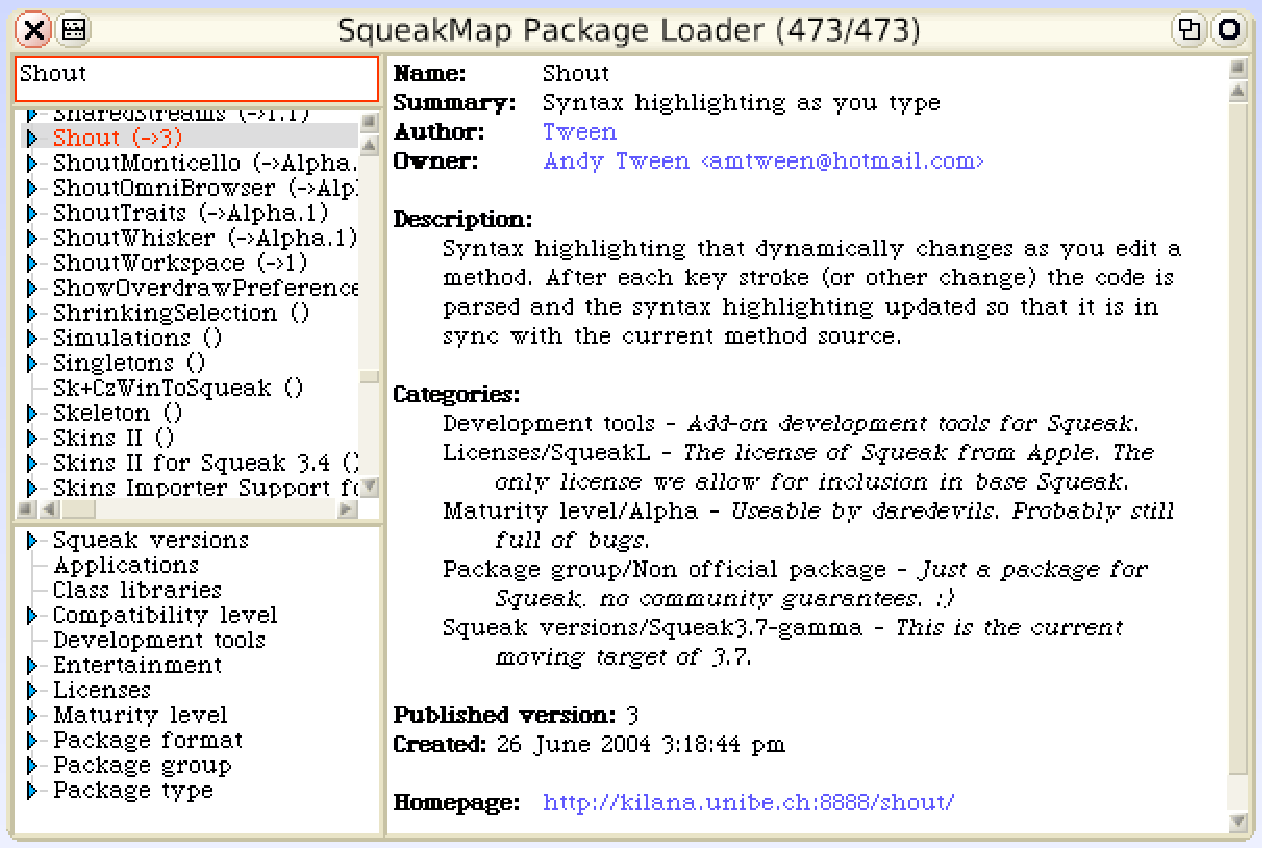
\includegraphics[width=10cm]{SM}
\caption{SqueakMap Package Loader on Shout    \label{sm}}
\end{center}
\end{figure}


\begin{enumerate}
\item Monticello: Monticello is a package support for Squeak (normally already included in 3.7 full release).
\item Shout (syntax highlighter while typing), 
\item KomHttpServer (web server): answer yes to the first two questions, and then \textbf{always} no,
\item Seaside (the dynamic web application framework): it asks you for a login and password,
\item Refactoring Browser for Squeak 3.7. 
\end{enumerate}


\section{Monticello}
Monticello is a CVS-like tool for Squeak. You can find the documentation at: \ct{http://www.wiresong.ca/Monticello/UserManual/}. Open Monticello using open... Monticello. Monticello allows you to save projects in various kind of servers: http, ftp, file system, data bases, \ldots. You can save your project on SqueakSource, if you want (\texttt{http://www.squeaksource.com}).

By convention, the name of a package should be the same as a class-category. As in Smalltalk this is possible to extend classes, you can associate a class extension with a package by putting a * followed by the name of the package in the method category. For example in Figure~\ref{mcbrowser}, the method named \ct{stylerAboutToStyle:} is defined in the \ct{*Shout-Styling} category, therefore it belongs to the package \ct{Shout-Styling}.

You can browse the contents of a package by clicking on the browse button and in particular  you can see the extensions associated to a package. See the Monticello chapter. 

\begin{figure}[h]
\begin{center}
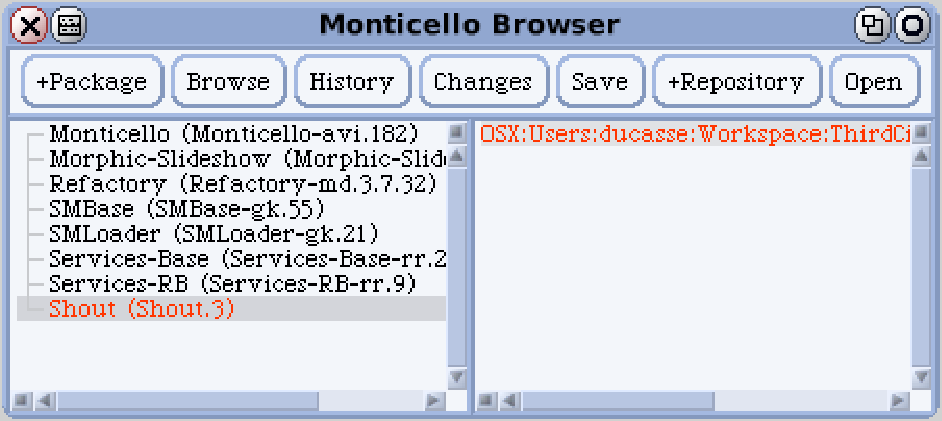
\includegraphics[width=10cm]{MC}
\caption{Monticello \label{}}
\end{center}
\end{figure}

\begin{figure}[h]
\begin{center}
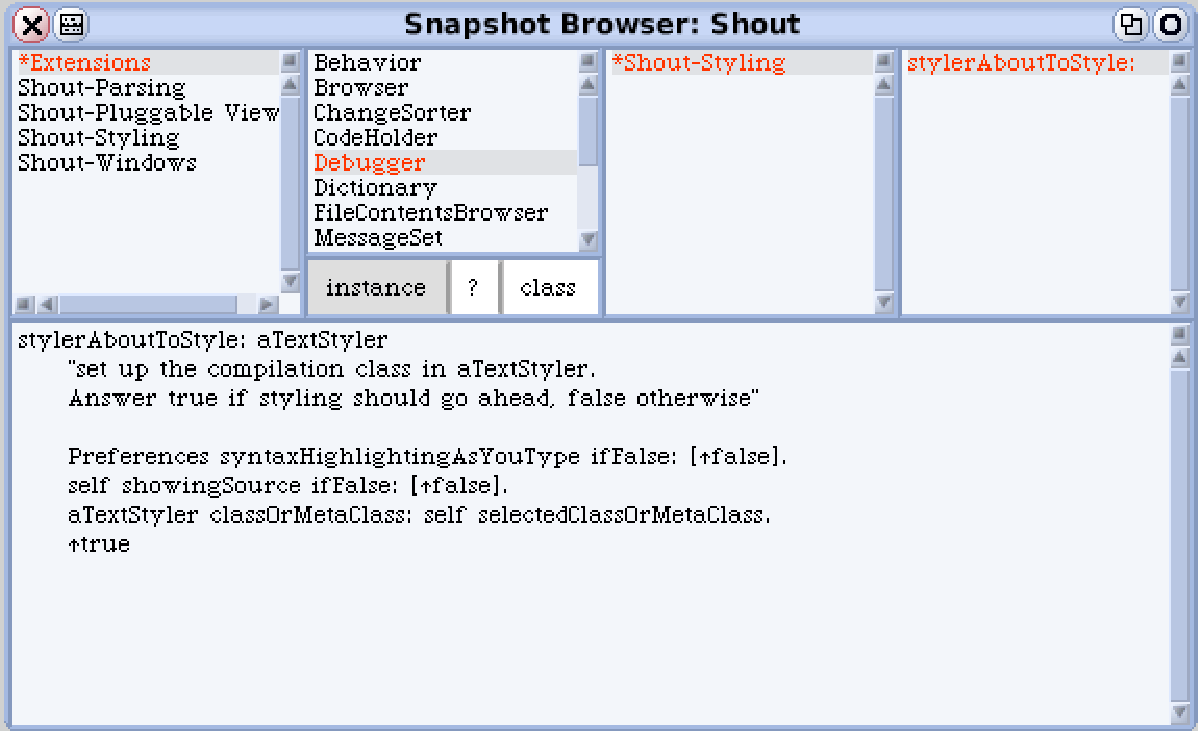
\includegraphics[width=8cm]{MCBrowser}
\caption{Browsing the changes associated to a package. \label{mcbrowser}}
\end{center}
\end{figure}

\section{SqueakSource: the Squeak SourceForge}

SqueakSource (\ct{www.squeaksource.com}) is a free source forge like open-source code repository. You can manage your squeak source there. For that you should define a project there and add it into your Monticello list of repositories. 

\begin{figure}[h]
\begin{center}
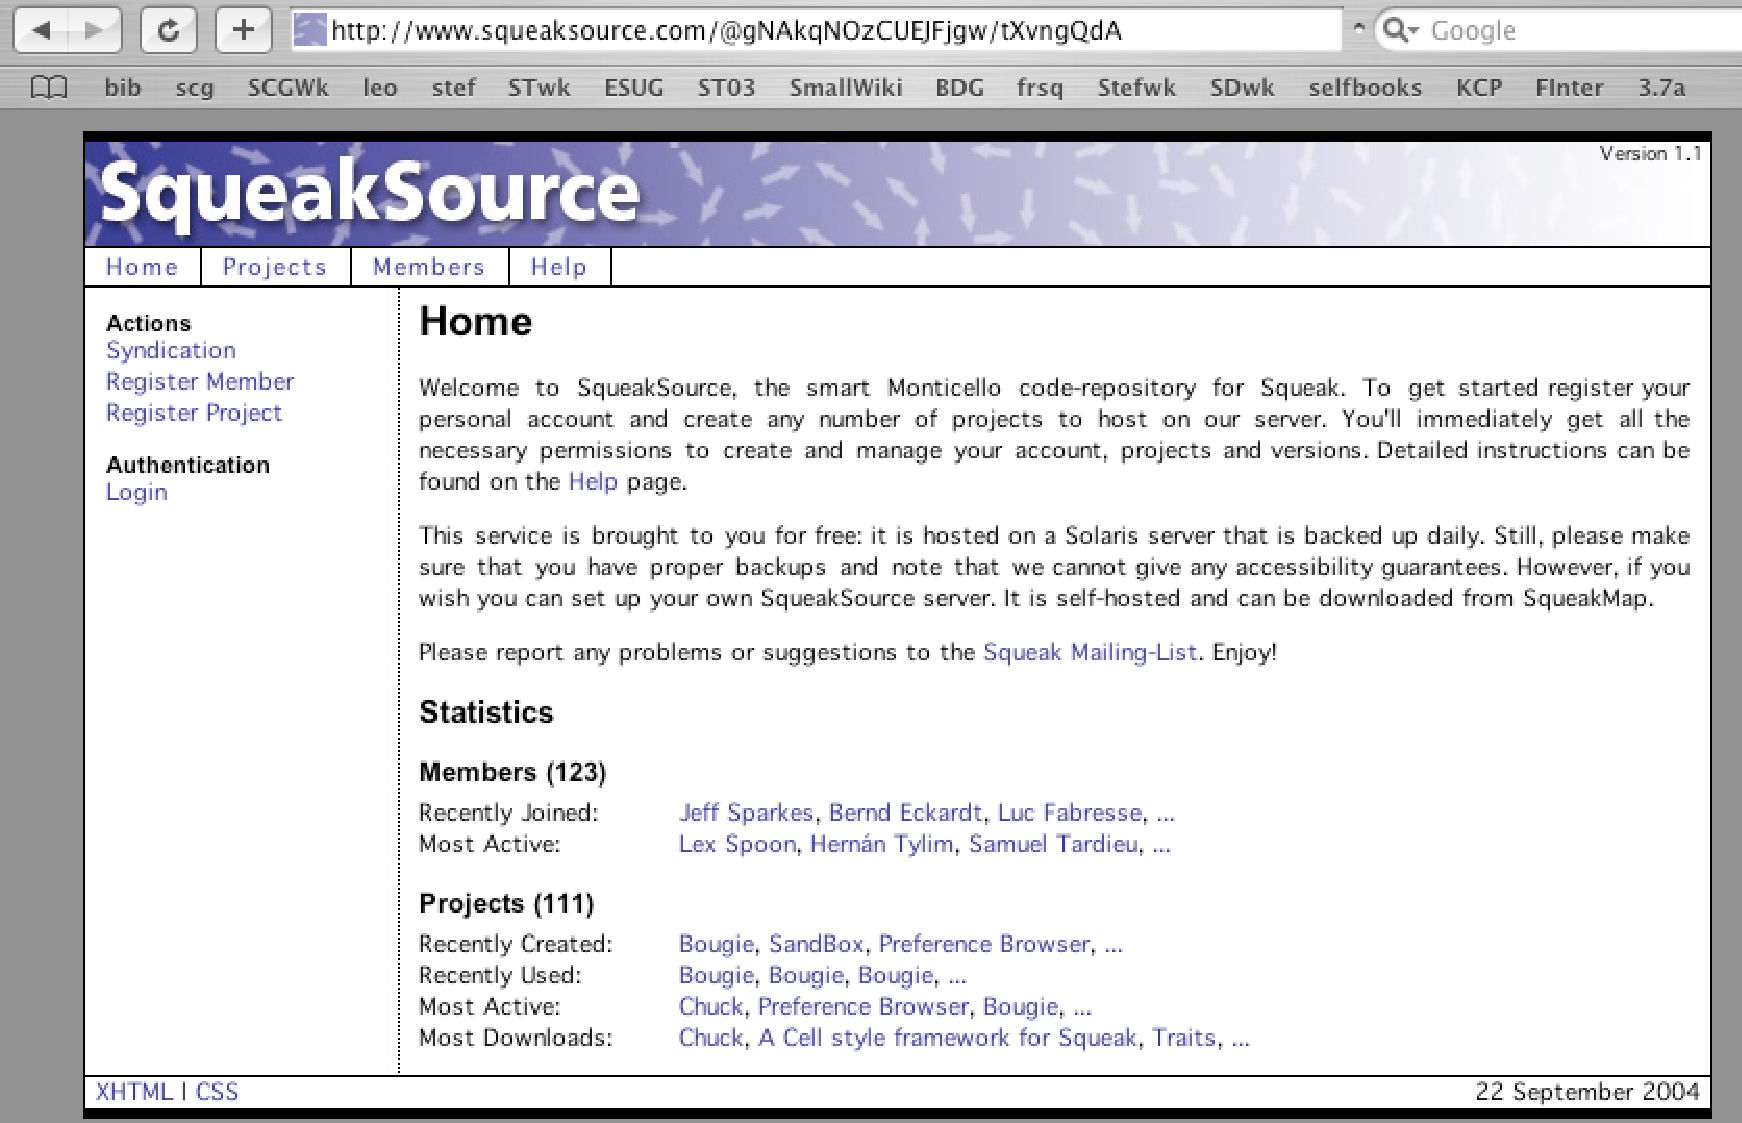
\includegraphics[width=15cm]{SqueakSource}
\caption{SqueakSource is a source forge like server for Squeak.\label{}}
\end{center}
\end{figure}

You can define a new repository in Monticello and publish automatically to this repository.
For that you should paste the project information specified in SqueakSource into the repository dialog as shown in Figure~\ref{SSrepo}
\begin{figure}[h]
\begin{center}
\includegraphics[width=10cm]{SSrepo}
\caption{Adding a repository to your monticello repository list.\label{SSrepo}}
\end{center}
\end{figure}


 \chapter{Monticello}

\section{Packages in Monticello: PackageInfo}

The PackageInfo system is a simple, lightweight way of organizing Smalltalk source: it is nothing more than a naming convention, which uses (or abuses) the existing categorization mechanisms to group related code. Let me give you an example: say that you are developing a framework named SqueakLink to facilitate using relational databases from Squeak. You will probably have a series of system categories to contain all of your classes (e.g., category \cat{SqueakLink-Connections} containing the classes \cls{OracleConnection}, \cls{MySQLConnection} and \cls{PostgresConnection})
(\cat{SqueakLink-Model} containing \cls{DBTable}, \cls{DBRow}  and \cls{DBQuery}) and so on. But not all of your code will reside in these classes - you may also have, for example, a series of methods to convert objects into an SQL friendly format: \cod{Object\di{}asSQL},  \cod{String\di{}asSQL} and  \cod{Date\di{}asSQL}.

These methods belong in the same package as the classes in \cat{SqueakLink-Connections} and \cat{SqueakLink-Model}. You mark this by placing those methods in a method category (of \cls{Object}, \cls{String}, \cls{Date}, and so on) named \cat{*squeaklink} (note the initial star). The combination of the \cat{SqueakLink-...} system categories and the \cat{*squeaklink} method categories forms a package named "SqueakLink".

The rules, to be precise, are this: a package named "Foo" contains

\begin{itemize}
\item All class definitions of classes in the system category \cat{Foo}, or in system categories with names starting with "Foo-".
\item All method definitions in any class in method categories named \cat{*foo} or with names starting with \cat{*foo-}.
\item All methods in classes in the system category \cat{Foo}, or in system categories with names starting with \cat{Foo-}, except those in method categories with names starting with \cat{*} (which must belong to other modules).
\end{itemize}

\section{Getting Started}

\paragraph{Installing}

The best way to install Monticello is via SqueakMap. Note however, that MC has two dependencies, both are part of the standard image, so it's usually not necessary to install them explicitly. However, the update stream tends to lag behind the versions on SqueakMap, so it's often a good idea to upgrade them before installing MC.!
\begin{itemize}
\item PackageInfo groups classes and methods into packages using a simple naming convention. It became part of the standard image in update 5250.
\item MCInstaller provides a way to load Monticello Versions into an image that doesn't have Monticello installed. Since Monticello is self hosting, it's used for bootstrapping. It's present in images updated through 5710 and later.
\end{itemize}

\paragraph{Creating a Working Copy}

Once Monticello is installed, the Monticello Browser will be available from the 'open...' menu. Open it by selecting World / open... / Monticello Browser.

The first thing you need to do is tell Monticello about the package you are interested in versioning. You do this by creating a Working Copy.

\paragraph{From an .mcz version file}
Open a FileList and navigate to the version file. Click on the 'Load' button to load the package into your image.

\paragraph{From a version in a repository}

First connect to the repository, either local or remote, that contains the verison you want to load. See below for details. Then open the repository: select the repository in the list on the right-hand side of the Monticello Browser, and click the 'Open' button. This will open a Repository Inspector. Select your version and click the 'Load' button.

\paragraph{From scratch}

Click on the '+Package' button, and enter the name of a PackageInfo package. It doesn't matter whether or not the code for the package already exists.

Once the Working Copy has been created, the name of the package will appear in the package list on the left side of the Monticello Browser. If you loaded an existing version, the version name will be displayed in parenthesis after the package name, otherwise the parenthesis will be empty, indicating that your working copy has no ancestors.

\paragraph{Connecting to a Repository}

If you've already got a Working Copy, click on the package name on the left side of the Monticello Browser, so that your repository will be associated with your package. To connect to a repository, click on the '+Repository' button in the Monticello Browser. A pop-up menu will appear, allowing you to select the type of repository you want to connect to.

The simplest repository type is 'directory.' When you select this type of repository, Monticello will open a FileList2 to allow you to select an existing directory in which to store versions. Other types of repositories typically require more configuration, and will open a text pane to allow you to enter it.

\paragraph{Saving Changes}

Changes to your working copy are automatically logged in your changes file, so you only need to create a new version of your package when you want to share the changes with others. Select the package on the left side of the Monticello Browser and the repository to save to on the right, then click the 'Save' button. See Repositories for discussion of how to publish to shared repositories.

\paragraph{Merging Changes}

If you or some other developer have made changes to the same version of a package, load one version as your working set and then select the repository containing the other version in the Monticello Browser, open a Repository Browser and select the other version. Clicking the 'Merge' button will automatically load all non-conflicting changes from the other version. If you need to control which changes to accept, you may instead click 'Changes' to browse every difference.



\section{Elements of Monticello}

\paragraph{Packages}

Packages are the units of versioning used by Monticello; the classes and methods they contain are recorded and versioned together. Monticello uses the packages defined by PackageInfo.

\paragraph{Snapshots}

A Snapshot is the state of a Package at a particular point in time

\paragraph{Versions}

A Version is a Snapshot of a Package and it's associated metadata - author initials, the date and time the snapshot was taken, and the Version's ancestry - the list of Versions from which it is derived.

A Version is the standard currency of the system. You save them, load them, give them to others, merge them, delete... you get the picture. Versions are often stored in mcz files - see File Format

\paragraph{Working Copies}

Each package in an image that is being versioned with Monticello has a Working Copy. The Working Copy represents the Version of the package that is currently active in the image, and which may be modified by the Smalltalk development tools.

\paragraph{Repositories}

These are places to store your Versions. Unlike CVS, in which a Package is associated with one Repository, a Monticello Package can have Versions in many repositories. When adding a new Repository to use, you can choose from SqueakMap Cache, FTP, HTTP (webdav), SqueakMap Release, SMTP, or a directory somewhere on your hard drive (or network drive).

For example, if I have six versions of package Foo, I could have Foo versions 1-4 being on my local harddrive, and 5-6 being on an ftp server. You could download version 5, make some changes and commit a new version (7) to your WebDAV repository. I can download and merge that version with my own work to produce version 8, which I save to my ftp repository.

This is a key element of Monticello's distributed development model.

\paragraph{Package cache}

The package-cache is a local repository the Monticello uses to cache any package that is loaded into a particular image in a directory. That means it is filled with .mcz files, whether it is a package you create in your image, or one you download from somewhere else.

When you use images in different directories you will have multiple package-caches, and may hold many of the same packages. If MC is loaded into an image which is subsequently moved, MC will continue to use the package-cache in the directory the image was moved from. Otherwise MC creates a new package-cache in the local directory. This can become a real mess and so some have used symlinks on unix systems to centralize it.

\paragraph{Why cache packages at all?}

When a Version is loaded into the image, it is likely to become the ancestor of new versions that are created as part of the development process. During merges, Monticello needs to examine the Snapshots of these ancestors in order to detect conflicts. By caching these ancestors as it loads them, MC reduces the chance that the necessary version will be unavailable - either because the repository it's in is no longer available or because it was loaded directly from a file and isn't in any repository.



\section{Repositories}

There are currently 8 types of repositories, each with different characteristics and uses. Repositories can be read-only, write-only or read-write.

\paragraph{HTTP}

HTTP Repositories are often general purpose read-write repositories for day-to-day development using a shared server. (Although the server can be configured for read-only access. Saving Versions via HTTP uses the PUT method, wich must be enabled on the server.)

The nice thing about HTTP repositories is that it's easy to link directly to specific versions from web sites or SqueakMap. With a little configuration work on the HTTP server, HTTP repositories can be made browseable by ordinary web browsers, WebDAV clients, etc.

\paragraph{FTP}

Similar to an HTTP repository, except that it uses an FTP server instead.

\paragraph{GOODS}

This repository type stores Versions in a GOODS object database. It's a read-write repository, so it makes a good "working" repository where Versions can be saved and retreived. Because of the transaction support, journaling and replication capabilities of GOODS, it is suitable for large repositories used by many clients.

\paragraph{directory}

A directory repository stores Versions in a directory in the local filesystem. Since it requires very little work to set up, it's handy for private projects or disconnected development. The Versions in a directory repository can be uploaded to a public or shared repository at a later time.

\paragraph{SMTP}

SMTP repositories are useful for sending Versions by mail. When creating an SMTP repository, you specify an a destination email address. This could be the address of another developer - the package's maintainer, for example - or a mailing list such as squeak-dev. Any Versions save to the repository will be emailed to this address.

\paragraph{SqueakMap Release}

This is a write-only repository used for publishing releases of a package to SqueakMap. To configure the repository enter the name of the package on SqueakMap, your SM initials and your SM password. Now any Versions saved to the repository will be uploaded to your SM account, and registered as a new release with SqueakMap.

\paragraph{SqueakMap Cache}

When packages are installed through SqueakMap, the downloaded files are stored in a cache. In order to make these files, which are often Versions in .mcz format, available to Monticello for loading, merges etc, a SqueakMap Cache repository is created when these files are loaded for the first time.

\paragraph{package-cache}

The package cache is a special repository that Monticello creates automatically. Like a directory repository, the package cache stores files in a directory on your local filesystem. See Elements of Monticello for more information.


\section{File Format}

Versions are often saved in binary files for storage in repositories, distribution to users etc. These files are commonly call 'mcz files' as they carry the extension .mcz.

\paragraph{Archive contents}

Mcz files are actually ZIP archives that follow certain conventions. Conceptually a Version contains four things:

\begin{itemize}
\item Package. A Version is related to a particular Package. Each mcz file contains a member called 'package' which contains information about the Version's Package.

\item VersionInfo. This is the meta-data about the Snapshot. It contains the author initials, date and time the Snapshot was taken, and the ancestry of the Snapshot. Each mcz file contains a member called 'version' which contains this information.
\item Snapshot. A Snapshot is a record of the state of the package at a particular time. Each mcz file contains a directory named 'snapshot/'. All the members in this directory contain definitions of program elements, which when combined form the Snapshot. Current versions of Monticello only create one member in this directory, called 'source.st'.
\item Dependencies. A Version may depend on specific Versions of other packages. An mcz file may contain a 'dependencies/' directory with a member for each dependency. These members will be named after the Package depended upon.
\end{itemize}

\paragraph{Source code encoding}

The member named 'snapshot/source.st' contains a standard fileout of the code that belongs to the package.

\paragraph{Metadata encoding}

The other memebers of the zip archive are encoded using S-expressions. Conceptually, the expressions represent nestable dictionaries. Each pair of elements in a list represent a key and value. The following example needs little explaination:

(key1 'value1' key2 (sub1 'sub value 1'))

\paragraph{Distributing mcz files}

The metadata for a Version ends up being fairly compact, so it's not unreasonable to distribute with a release. It's also important that it be present if somebody decides to start hacking on your Package. Then they can create a mcz with their Version of your package and it will have the correct ancestry information, enabling you to easily and correctly merge it back into your work.

Stated another way, a Version doesn't contain a full history of the source code. It's a snapshot of the code at a single point in time, with a UUID identifying that snapshot, and a record of the UUIDs of all the previous snapshots it's descended from. So it's a great thing to distribute.

\section{The Monticello Browser}

The Monticello Browser is the central window of the interface. All versioning operations begin with the Monticello Browser.

The browser contains two panes. The left pane contains the list of packages that have Working Copies in the image. In parenthesis, the immediate ancestors of the Working Copies are also listed. Packages that have been modified since they were loaded are displayed with an asterisk before their names. The list on the right shows the repositories that are configured for the selected package. The buttons across the top are enabled and disabled depending on the selections in the two panes; many commands require you to first select a package and repository.

\paragraph{+Package}

The '+Package' button is used to create a Working Copy for a package. When you click on it, Monticello will ask for the name of the Package you want to version, the same name that PackageInfo uses to identify the package. Once the Working Copy has been created, the name of the package will appear in the left pane.

The '+Package' button should only be used to create a Working Copy for a brand-new package, one that has not previously versioned with Monticello. To create a Working Copy from an existing Version, you should load the version from a repository or directly from an .mcz file using the FileList. See Getting Started for details.

\paragraph{Browse}

The 'Browse' button takes a Snapshot of the current state of the selected package and opens a Snapshot Browser on it.

\paragraph{History}

The 'History' button opens a History Browser on the Working Copy for the selected pacakge.

\paragraph{Changes}

The 'Changes' button is used to display the changes made to the selected package since it was last saved or loaded. Monticello first takes a Snapshot of the package and compares it to the package's first immediate ancestor. If any changes have been made, a Patch Browser is opened to display them.

\paragraph{Save}

The 'Save' button is for saving new Versions of the selected package. It opens a dialog that allows you to enter the name of the new version and a log message describing the changes made since the last version. If you click 'accept,' Monticello will take a Snapshot of the package and save it as a Version to the selected repository.

\paragraph{+Repository}

The '+Repository' button is used to connect to a Repository. It opens a menu allowing you to choose the type of repository you with to connect to, and depending on the repository type, a configuration dialog for the connection.

\paragraph{Open}

The 'Open' button opens a Repository Inspector on the selected repository. The is useful when you need to find a specific Version to load, merge, browse etc.

\section{The Snapshot Browser}

The Snapshot browser is much like the standard Smalltalk System Browser except that it displays the contents of a Snapshot, rather than the code that is active in the image. Since Snapshots are immutable, the Snapshot browser does not allow editiing.

One difference between the Snapshot Browser and the familiar system browsers is that the Snapshot browser uses the special system category '*Extensions' to categorize classes that do not belong to the package, but which have extension methods that do.

\section{More on PackageInfo}
To get a feel for this, try filing the Refactoring Browser. The Refactoring Browser code uses PackageInfo's naming conventions, using "Refactory" as the package name. In a workspace, create a model of this package with  \cod{refactory := PackageInfo named: 'Refactory'}. 

It is now possible to introspect on this package; for example, refactory classes will return the long list of classes that make up the Refactoring Browser. refactory coreMethods will return a list of MethodReferences for all of the methods in those classes. refactory extensionMethods is perhaps one of the most interesting queries: it will return a list of all methods contained in the Refactory package but not contained within a Refactory class. This includes, for example, \cod{String\di{}expandMacrosWithArguments:} and \cod{Behavior\di{}parseTreeFor:}.

Since the PackageInfo naming conventions are based on those used already by Squeak, it is possible to use it to perform analysis even of code that has not explicitly adapted to work with it. For example, (PackageInfo named: 'Collections') externalSubclasses will return a list of all Collection subclasses outside the Collections categories.

You can send fileOut to an instance of PackageInfo to get a changeset of the entire package. For more sophisticated versioning of packages, see the Monticello project.






\ifx\wholebook\relax\else\end{document}\fi
